\documentclass[xcolor=dvipsnames]{beamer}

\usetheme{Boadilla}

\newcommand{\bi}{\begin{itemize}}
\newcommand{\ei}{\end{itemize}}
\newcommand{\be}{\begin{enumerate}}
\newcommand{\ee}{\end{enumerate}}
\newcommand{\bc}{\begin{center}}
\newcommand{\ec}{\end{center}}
\newcommand{\I}{\item}
\newcommand{\f}{\frame}
\newcommand{\ft}{\frametitle}

\title{Overview of GlueX Offline Computing}
\subtitle{Spring Meeting of the APS, Garden Grove, California}
\author[M.\ Ito]{Mark M.\ Ito}
\date{April 30, 2011}
\institute[JLab]{Jefferson Lab}

\begin{document}

\f{\titlepage}

\f{
\ft{GlueX in Hall D at Jefferson Lab}
\bc
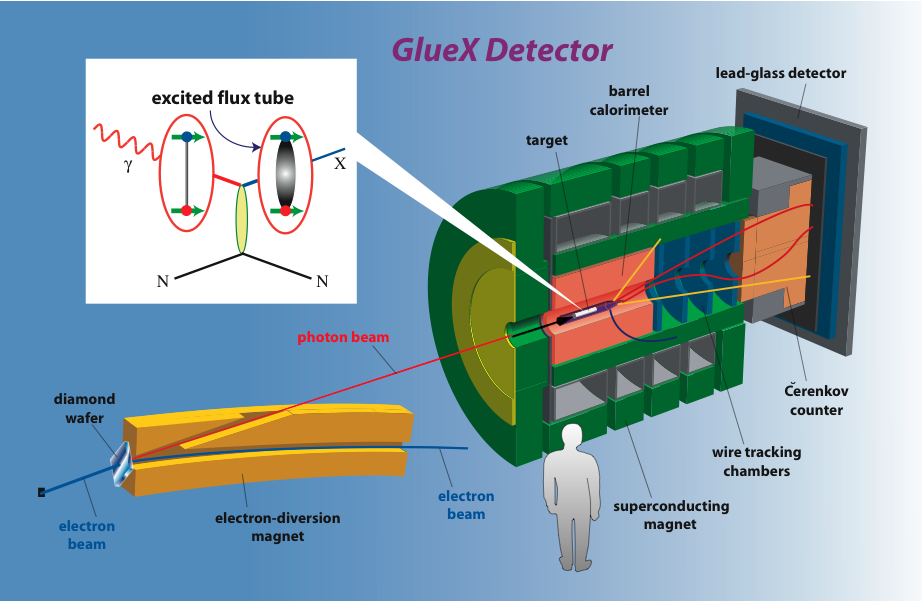
\includegraphics[height=3.0in]{detector.png}
\ec
}

\f{
\ft{Geometry}
  \bi
  \I Implemented in XML
  \I Hall D Detector Specification (HDDS)
  \I XML elements and attributes closely follow GEANT defined shapes and their parameters
  \I Goal: keep the geometry in one place, use in
    \bi
    \I Simulation
    \I Reconstruction
    \I Event display
    \ei
  \ei
}

\f{
\ft{Simulation}
\bi
\I GEANT3-based: HDGEANT
  \bi
  \I Geometry information auto-coded into FORTRAN code from HDDS information
  \I Hits ({\it i. e.}, digitization) coded separately
  \I Output in Hall Data Description Model format (HDDM, see slide below)
  \ei
\I Experimental resolution added in separate stage: mcsmear
  \bi
  \I HDDM in, HDDM out
  \ei
\I Effort started to transition to GEANT4
\ei
}

\f{
\ft{Reconstruction}
\bi
\I JANA
  \bi
  \I multi-threaded: each thread a separate event stream
  \I algorithms for different detectors implemented as "factories"
  \ei
\I ROOT used for some general utilities
\I Hooks for user code
  \bi
  \I user's class inherits from abstract base class
  \I must be registered with the framework
  \I multiple user classes possible
  \ei
\I Plug-in mechanism
  \bi
  \I e. g., define user class at run time
  \ei
\ei
}

\f{
\ft{Partial Wave Analysis (PWA)}
\bi
\I Achieving physics goals of GlueX depends critically on PWA.
\I Collaborative Research: Open Access Amplitude Analysis on a Grid
  \bi
  \I NSF-funded effort
  \I Carnegie Mellon, Indiana, Connecticut
  \ei
\I AmpTools 
  \bi
  \I PWA toolkit
  \I Indiana University
  \ei
\I Ruby-PWA
  \bi
  \I PWA toolkit
  \I Carnegie Mellon University
  \ei
\ei
}

\f{
\ft{Calibration Database}
\bi
\I Relational database
\I Based on CLAS experience (Hall B, JLab) with improvements
\I Complete version history, with version choice at API level
\I Facility for private versions, with history
\I Tagging facility
\I Interfaces:
  \bi
  \I C++ API
  \I Web
  \I Command line
  \I Unix-like shell (CCDB shell) for browsing directory structure
  \ei
\I Technology
  \bi
  \I MySQL
  \I C++
  \I JQuery
  \I Python
  \ei
\ei
}

\f{
\ft{Data Format}
\bi
\I Raw data: EVIO
  \bi
  \I native CODA format
  \ei
\I Simulation output: HDDM
  \bi
  \I Hall Data Description Model
  \I A compressed XML
  \I Retains schema-like template at beginning of each file (uncompressed)
  \I C-based API
  \I C++ API in testing
  \ei
\I Reconstruction output:
  \bi
  \I HDDM
  \I EVIO
  \I ROOT trees
  \ei
\ei
}

\f{
\ft{Utilities}
\bi
\I XML parsing: Xerces
\I Source code management: subversion
\I Source code documentation: doxygen
\I Building scripts: GNU Make
\I Database: MySQL
\I General documentation
  \bi
  \I GlueX Notes: DocDB
  \I Webpages: mediawiki
  \ei
\ei
}

\f{
\ft{Computing}
\bi
\I Simulation
  \bi
  \I Use member institutions' resources
  \I Grid
  \I Effort has started
  \ei
\I Reconstruction
  \bi
  \I Raw data: reconstruct on JLab Farm
  \ei
\I PWA
  \bi
  \I Grid
  \I GPU farms
  \ei
\ei
}

\f{
\ft{More info?}
\bc\Large
http://wiki.gluex.org \\
click on ``Offline Software''
\ec
}

\f{
\bc\Large
Slide Show
\ec
}

\f{
\ft{Hall D, CEBAF, Jefferson Lab, exterior}
\bc
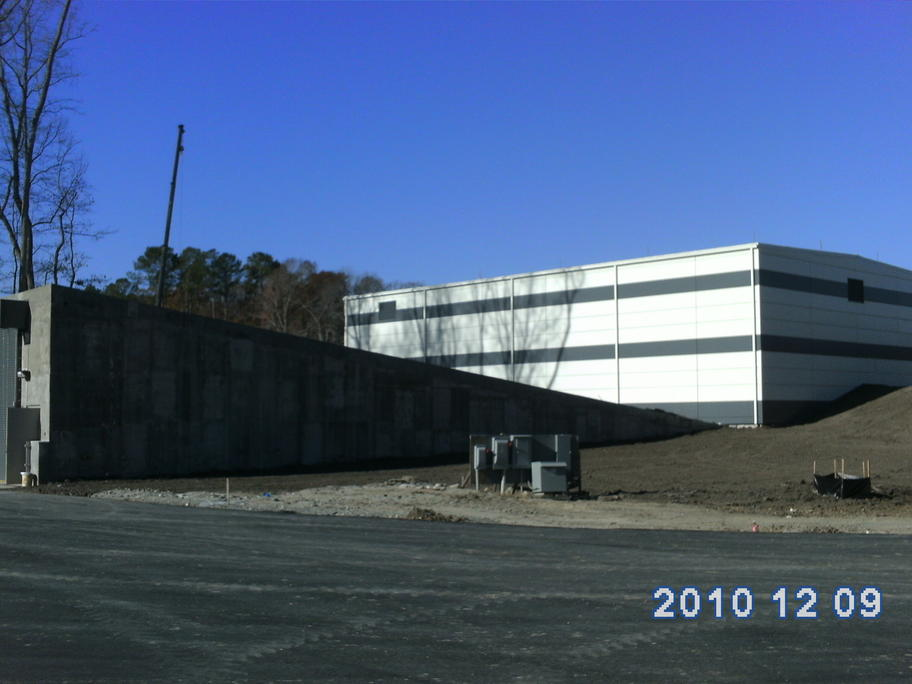
\includegraphics[height=3.0in]{hall_outside.jpg}
\ec
}

\f{
\ft{Hall D, CEBAF, Jefferson Lab, interior}
\bc
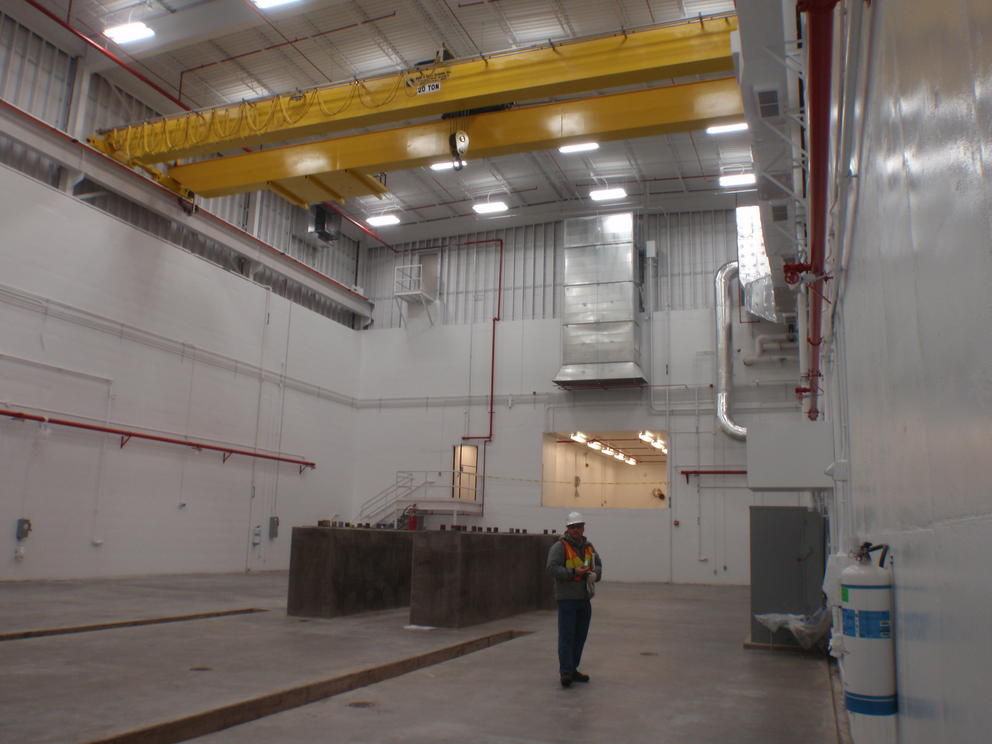
\includegraphics[height=3.0in]{hall_inside.jpg}
\ec
}

\f{
\ft{test one coil of the superconducting solenoid}
\bc
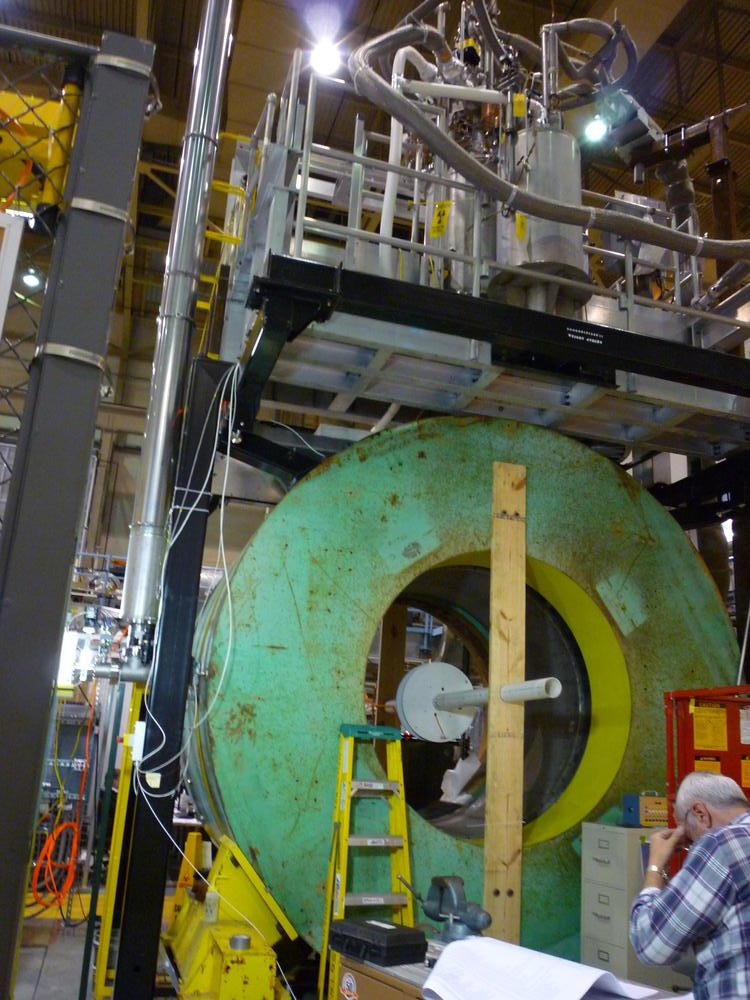
\includegraphics[height=3.0in]{magnet.jpg}
\ec
}

\f{
\ft{silicon photo-multipliers, for barrel calorimeter readout}
\bc
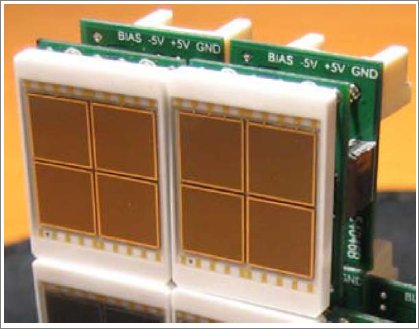
\includegraphics[height=3.0in]{sipm.jpg}
\ec
}

\f{
\ft{barrel calorimeter module}
\bc
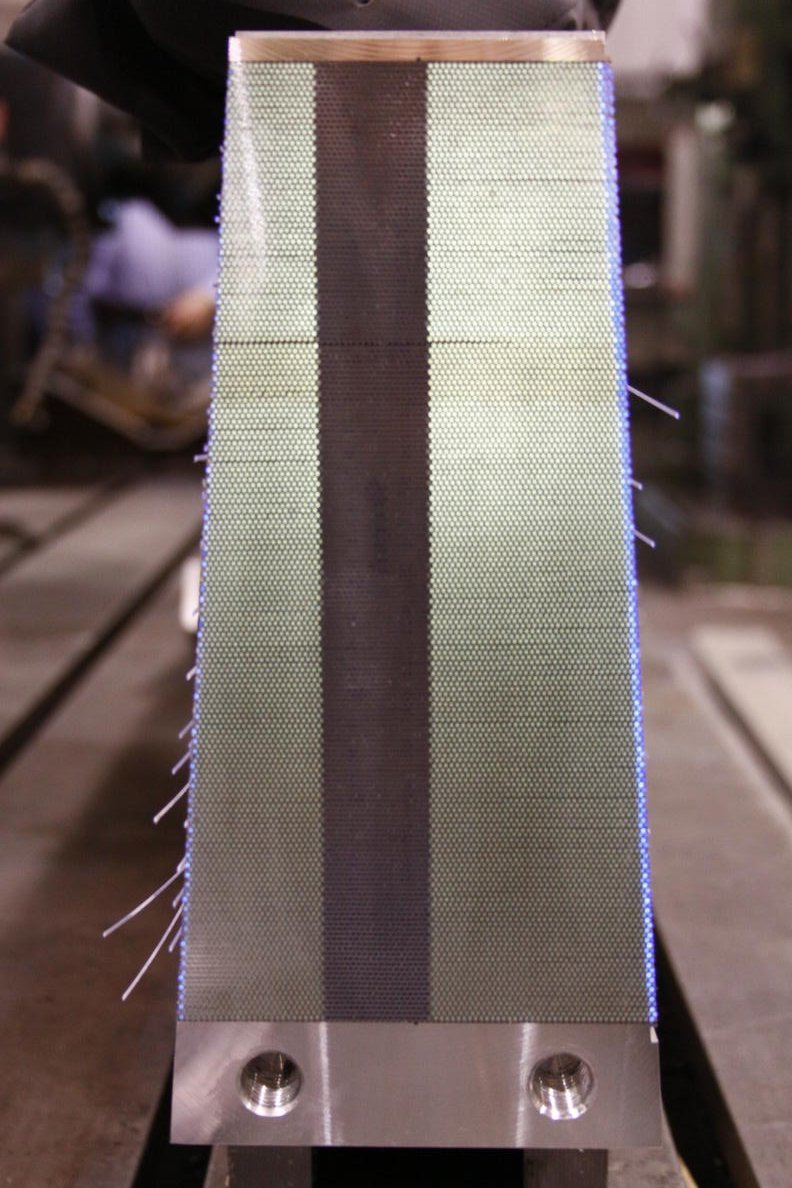
\includegraphics[height=3.0in]{bcal.jpg}
\ec
}

\f{
\ft{section of circular cathode foil, forward drift chambers}
\bc
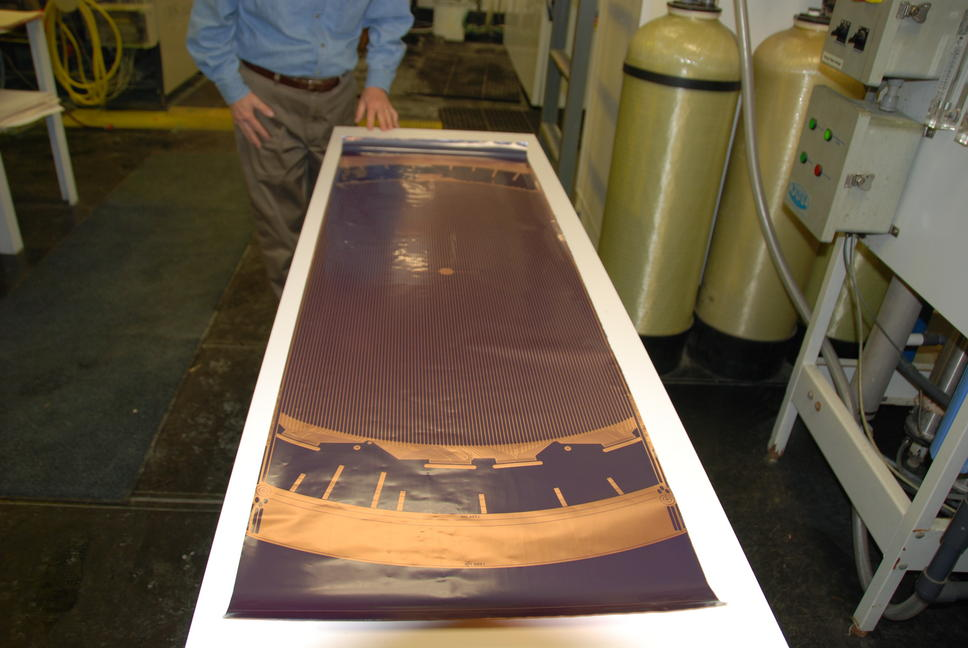
\includegraphics[height=3.0in]{cathode.jpg}
\ec
}

\f{
\ft{circuit board for forward drift chamber frame}
\bc
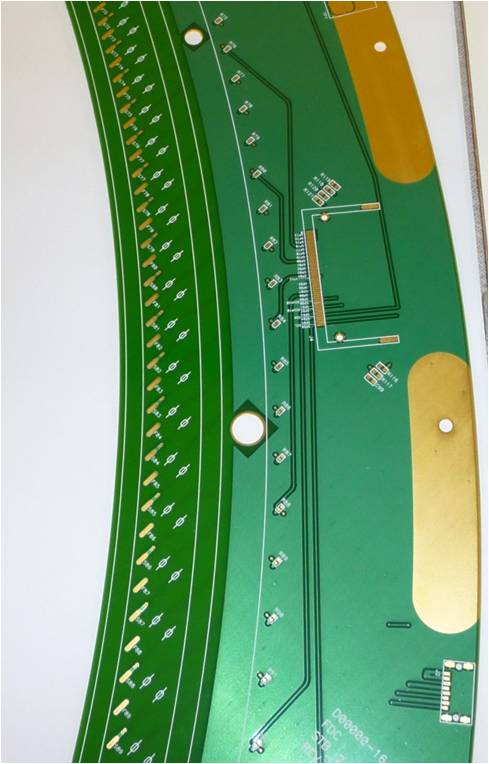
\includegraphics[height=3.0in]{fdc_board.jpg}
\ec
}

\f{
\ft{central drift chamber endplates + engineer}
\bc
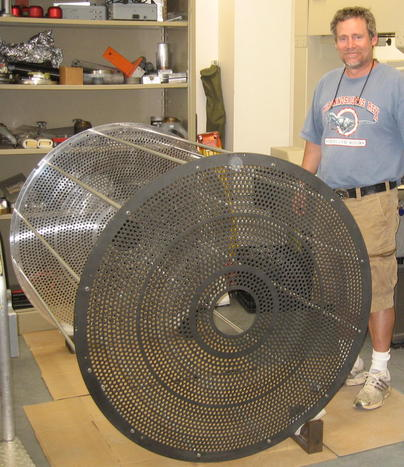
\includegraphics[height=3.0in]{cdc.jpg}
\ec
}

\f{
\ft{straw tubes, as shipped, for central drift chamber}
\bc
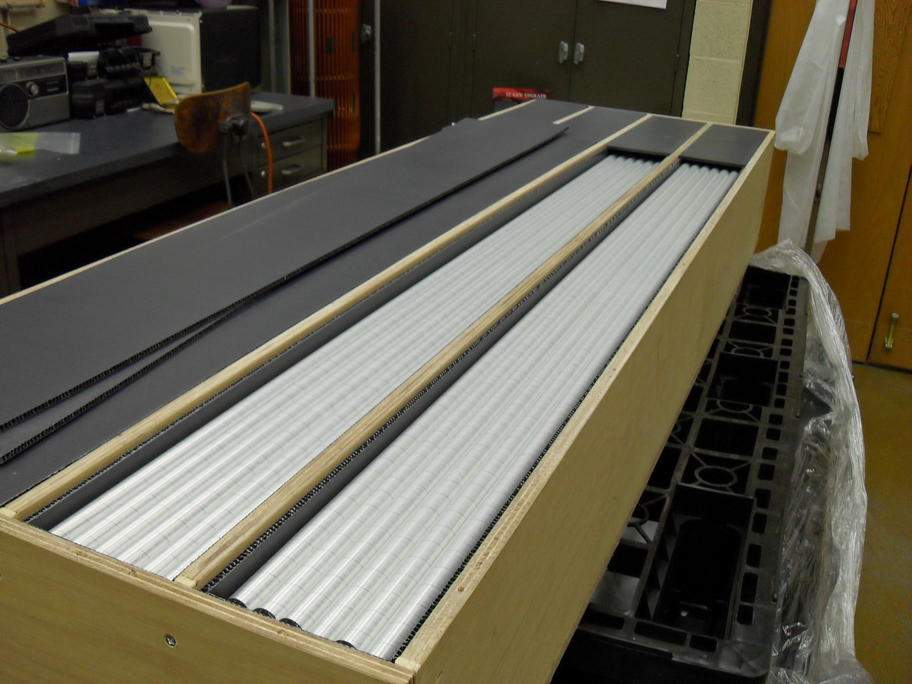
\includegraphics[height=3.0in]{straws.jpg}
\ec
}

\f{
\ft{straws being installed, central drift chamber}
\bc
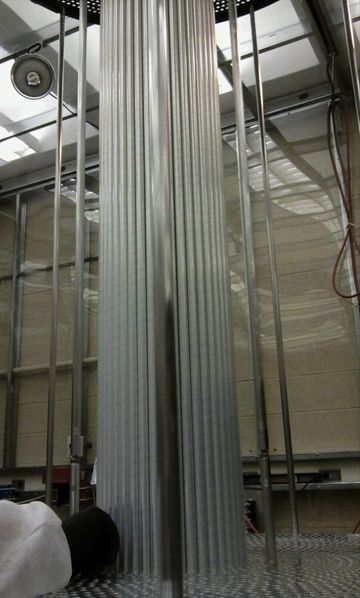
\includegraphics[height=3.0in]{straws_install.jpg}
\ec
}

\f{
\bc\Large
The End
\ec
}

\end{document}

% end of latex file
